\documentclass[11pt]{article}
\usepackage{amsmath,amsthm,amssymb}
\usepackage{graphicx}
\usepackage{fontspec}
\setmainfont{Arial}
\usepackage{wrapfig}
\usepackage[toc,page]{appendix}
\usepackage[font=footnotesize]{caption}
\usepackage[margin=0.5in]{geometry}
\usepackage[singlespacing]{setspace}
\usepackage[small, compact]{titlesec}  % http://ctan.mirrors.hoobly.com/macros/latex/contrib/titlesec/titlesec.pdf
\titleformat*{\subsubsection}{\slshape}
\usepackage{paralist}
\renewenvironment{thebibliography}[1]{
    \let\par\relax\let\newblock\relax
    \inparaenum[\bfseries{[}1{]}]}{\endinparaenum}
\usepackage[english]{babel}
\pagenumbering{gobble}
\usepackage{lineno}
%\linenumbers % remove before submitting

\begin{document} % 7 page limit
\sloppy
\begin{center}
\large{\textbf{
    Functional Activity of the Human Gut Microbiome to Classify Colorectal Cancer
}} \\
\vspace{11pt}
\small{
    Kelly L. Sovacool \\
    August 2020
}
\end{center}

\section*{Specific Aims} % 1 page

Changes in the taxonomic composition and metabolic activity of human microbiomes have been observed in several diseases.
In the case of colorectal cancer (CRC), evidence of toxigenic activity by gut microbes implies that these changes are not only a response to disease, but may also play a role in disease etiology.
Taxonomic composition is commonly defined by amplicon sequencing of the 16S rRNA gene and clustering sequences into Operational Taxonomic Units (OTUs).
Previous studies have built OTU-based machine learning models to classify stool samples as normal or cancerous, to serve as a less invasive diagnostic tool for CRC than colonoscopy.
Efforts to find consistent changes in taxonomic composition of microbiomes between normal and dysbiotic states have found mixed success, in part because interpersonal variability in taxonomic composition sometimes exceeds the variability between disease states.
Variability of microbiome composition between individuals with the same disease status may be explained by functional redundancy, where different microbial species carry out the same functions and thus can replace each other with little effect on the overall function of the community.

Sequencing whole metagenomes to identify the genes present and annotate known gene functions is commonly used to build a profile of functional potential of the microbiome.
Combining taxonomic composition from OTUs with functional potential from metagenomes allows one to characterize functional redundancy across communities, where communities with similar functional potential have different taxonomic composition.
Untargeted mass spectrometry can validate the functional potential characterized from metagenomics by identifying metabolites that are active in a community, thus painting a more precise picture of active microbial functions.
Here, I propose to investigate the impacts of taking functional redundancy and active metabolites into account on human stool sample classification for CRC diagnosis.

\subsection*{Aim 1. Assess the impact of functional redundancy of the gut microbiome on CRC classification.}
\textit{Hypothesis: Using functional gene profiles instead of only taxonomic profiles improves the classification modeling of samples as CRC or non-cancerous because of functional redundancy in the gut microbiome.}
\begin{compactenum}[A.]
    \item Build taxonomic profiles with OTUs from 16S rRNA gene sequences and build profiles of functional gene potential from metagenomes.
    \item Compare taxonomic composition to functional gene potential of microbiomes within and between disease states to determine presence and degree of functional redundancy.
    \item Build machine learning models to classify samples as CRC or non-cancerous with taxonomic composition, functional gene potential profiles, or both as model features and compare performance.
\end{compactenum}

\subsection*{Aim 2. Assess the impact of integrating active metabolites with functional gene potential on CRC classification.}
\textit{Hypothesis: Using active metabolic pathways confirmed with mass spectrometry instead of all potential metabolic pathways from metagenomes improves the classification modeling of samples as CRC or non-cancerous.}
\begin{compactenum}[A.]
    \item Annotate compounds from untargeted mass spectrometry with the GNPS database and select those known to be products of bacterial metabolic pathways with the MetaCyc database.
    \item Calculate the intersection of pathways associated with active metabolites and the pathways from functional potential profiles from metagenomes.
    \item Build machine learning models to classify samples as CRC or non-cancerous with all potential metabolic pathways or only confirmed active metabolic pathways as model features and compare performance.
\end{compactenum}

\section*{Dataset}
Stool samples were collected from patients undergoing colonoscopy as part of the GLNE 007 study (https://clinicaltrials.gov/ct2/show/study/NCT00843375).
211 individuals were diagnosed with CRC and 223 were confirmed non-cancerous.
16S rRNA gene amplicon sequencing was performed and remaining stool was kept frozen.
Part of the remaining stool will be used for whole metagenome shotgun sequencing and untargeted tandem mass spectrometry to complete these aims.

\section*{Background and Motivation} % 1/2 - 1 page

After lung cancer, colorectal cancer is the cause of the most cancer-related deaths worldwide \cite{ferlay_cancer_2015}.
Genetic factors explain only a small proportion of CRC cases, and lifestyle-based factors such as diet and smoking status are common to many cancer types \cite{thomas_metagenomic_2019}.
Many studies have observed changes in the composition of the gut microbiome in CRC, implicating microbes as potential risk factors, or at least as signatures that change in response to CRC \cite{kostic_genomic_2012, chen_decreased_2013}.
Thus, there is great interest in identifying microbial biomarkers involved in CRC to improve our understanding of the disease and to develop improved diagnostic tests.
Experiments in mouse models have found that treating germ-free mice with fecal matter transplants from CRC patients accelerated the progression from adenoma to carcinoma \cite{li_gut_2019, sobhani_colorectal_2019}.
Additionally, toxigenic microbial gene products such as colibactin have been associated with human CRC gut microbiomes and experimentally tested as drivers of disease progression with mouse models \cite{cougnoux_bacterial_2014, gagnaire_collateral_2017, thakur_unveiling_2019}.
These findings imply that microbiome changes occur not only as a response to CRC,
but may actually play a causative role in disease etiology.

Whether the microbiome changes in response to CRC, plays a role in disease progression, or both,
microbial biomarkers hold promise as a potential diagnostic tool.
Colonoscopy is currently the most effective way to detect screen-relevant neoplasias (SRNs; adenomatous and cancerous lesions),
which can then be biopsied during the same colonoscopy session for diagnostic confirmation.
But despite its effectiveness, the cost and highly-invasive nature of colonoscopy cause low patient compliance \cite{ling_attitudes_2001, jones_patient-reported_2010}.
The fecal immunochemical test (FIT), a quantitative measure of hemoglobin concentrations in stool,
is currently the best non-invasive screening tool for SRNs, but has low sensitivity.
OTU-based machine learning (ML) models have been developed that modestly improve sensitivity when used in complement with FIT, demonstrating the feasibility of using microbiome-based markers for diagnosis \cite{baxter_microbiota-based_2016}.

\begin{wrapfigure}{R}{0.35\textwidth}
    \vspace{-11pt}
    \centering{
        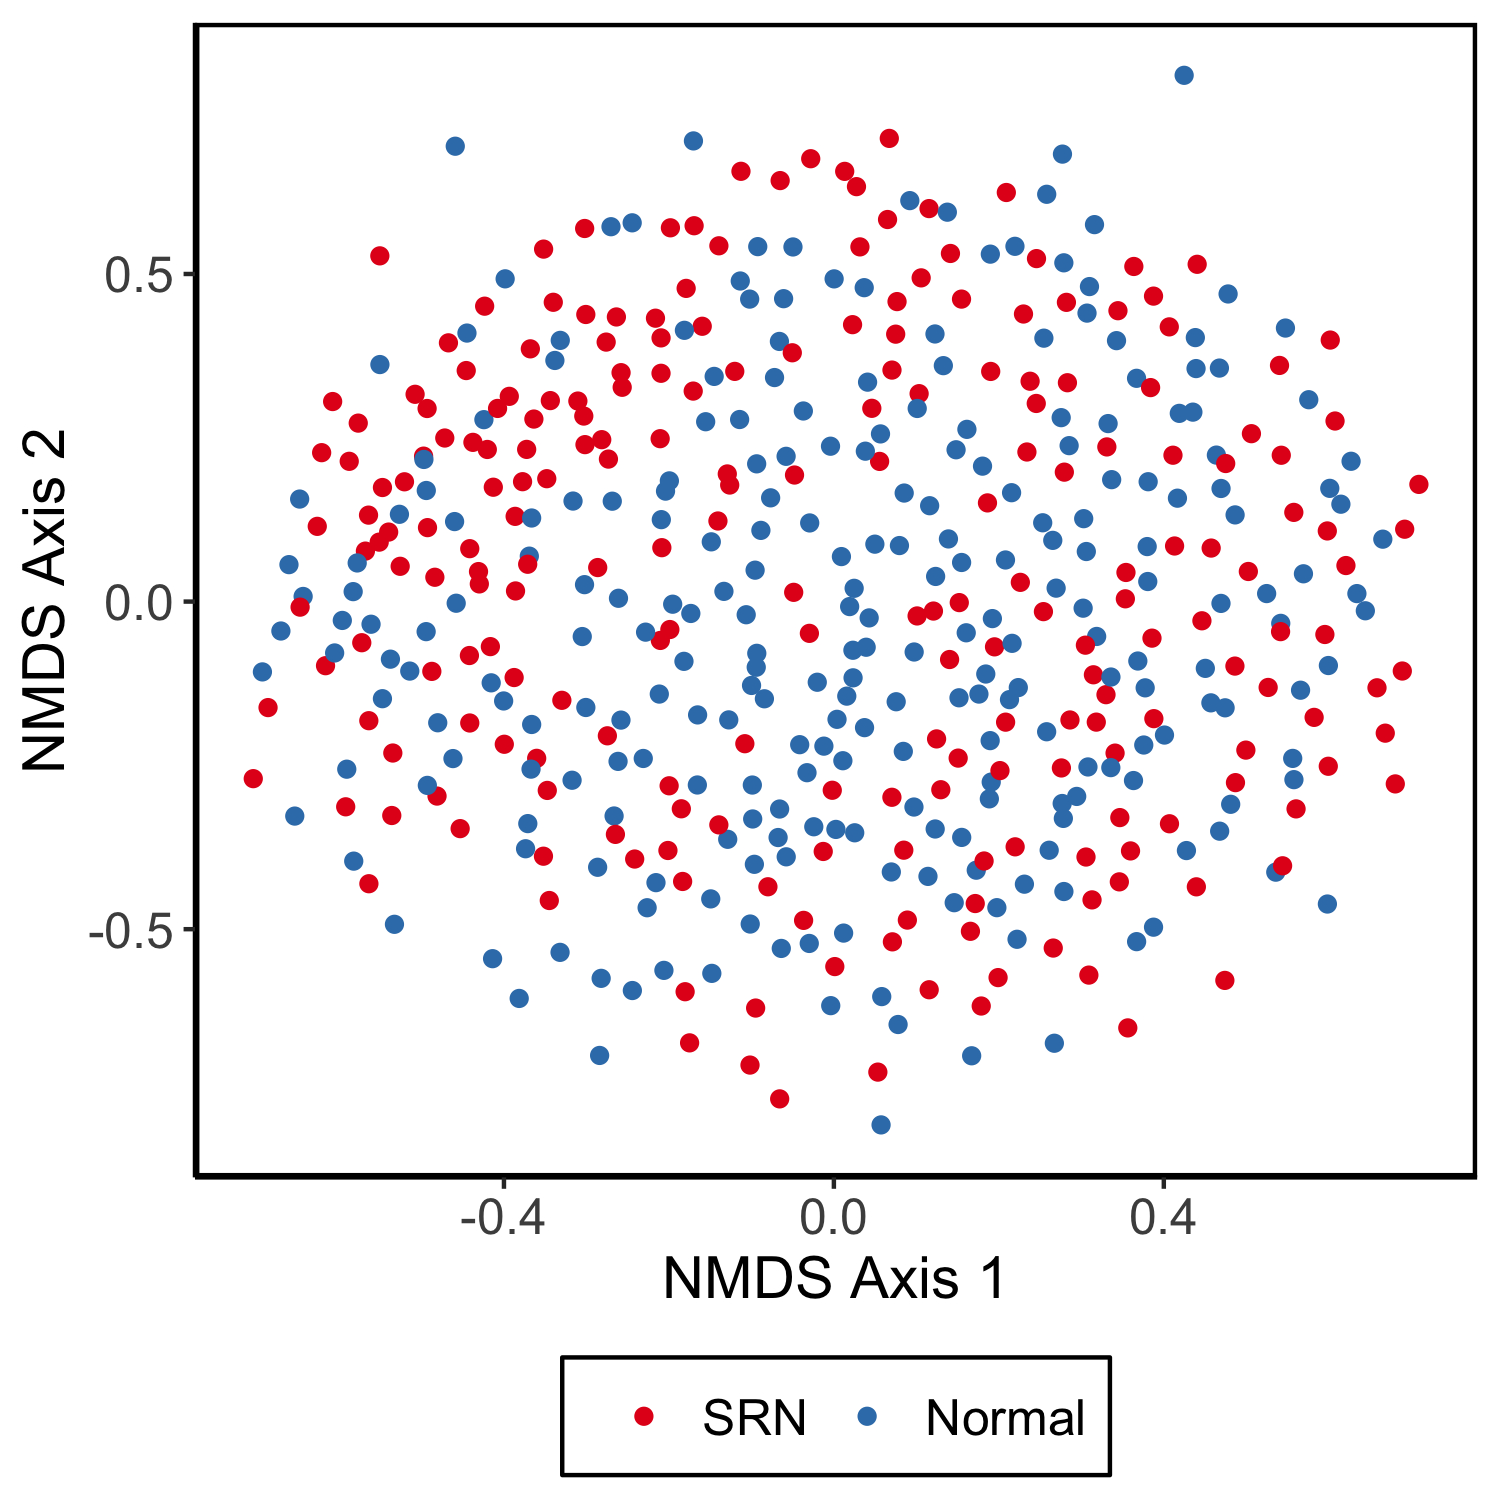
\includegraphics[width=0.35\textwidth]{figures/topcuoglu_s1.png}
        \caption{NMDS ordination of Bray-Curtis distances on fecal OTUs from 261 patients with normal colonoscopies and 229 patients with screen relevant neoplasias (SRN), which includes both adenoma and carcinoma. \cite{topcuoglu_framework_2020}}
        \label{fig:nmds_otu}
    }
    \vspace{-8pt}
\end{wrapfigure}
No single organism or gene has been indicated in all cases of CRC;
rather, the activities of the microbial community as a whole seem to be implicated \cite{louis_gut_2014}.
Taxonomic composition is often compared between ecological communities by calculating a beta diversity metric such as the Bray-Curtis dissimilarity, then plotting an ordination to visualize separation between disease states.
However, patient stool samples cannot be classified as having SRNs or not using beta diversity metrics,
as seen in the lack of distinct clustering of disease states shown in Fig. \ref{fig:nmds_otu}.
The reason is microbiome composition is highly variable between individuals, even more so than between disease states.
This finding has been observed not only across independent CRC datasets but also in other diseases including obesity and oral cancer \cite{weir_stool_2013, finucane_taxonomic_2014, perera_inflammatory_2018}.

It has been proposed that this interpersonal variability can be explained by the ability of different microbial species to carry out the same functions,
allowing communities with different taxonomic composition to cause the same disease \cite{franzosa_species-level_2018}.
Researchers are increasingly turning to whole-metagenome shotgun sequencing in order to explore the genes and build profiles of funtional potential of microbiomes.
Indeed, metagenomics studies have found some associations between specific potential functional pathways and CRC \cite{thomas_metagenomic_2019}.
Using functional potential profiles in addition to or in place of taxonomic composition may therefore improve the performance of classification models for CRC detection.

Functional redundancy is the phenomenon where different species carry out the same functions and thus can replace each other with little effect on the overall function of a community.
The concept of functional redundancy has been developed and explored in the field of ecology,
but few studies have directly applied it to microbial ecology specifically \cite{ricotta_measuring_2016}.
There does not seem to be a consensus on how to assess functional redundancy in culture-independent microbial communities,
where function is often measured indirectly using meta'omic approaches \cite{louca_function_2018, heintz-buschart_human_2018, tully_dynamic_2018, royalty_quantitative_2020}.
Many published studies claiming to have found functional redundancies in microbial systems lack quantitative analyses of redundancy,
instead vaguely describing patterns observed by eye \cite{souza_metagenomic_2015, ferrer_microbiota_2013, galambos_genome-resolved_2019}.
The problem is further complicated by the existence of slightly different competing definitions of functional redundancy.
Definitions from macroecology use species counts, rendering them not easily adaptable to meta'omics data which are inherently compositional.
Royalty \textit{et al.} very recently defined functional redundancy at the trait level as the evenness in relative contribution of a trait among taxa in a community \cite{royalty_quantitative_2020}.
Another definition which seems to be popular is that if different microbial communities have different taxonomic composition, but similar functional composition, there is functional redundancy \cite{louca_function_2018}.
This last heuristic has advantages:
1) it is defined by comparing different communities rather than within the same community, which easily links back to the motivating problem of interpersonal variability exceeding inter-disease state variability;
2) computational resources can be saved by comparing community compositions overall, rather than calculating a metric for every observed function in every community.
Finding evidence for functional redundancy in CRC and non-cancerous gut metagenomes would support the idea that functional redundancy can explain the high degree of interpersonal variability in microbiome composition.

It is important to note that metagenomics only shows the functional \textit{potential} of a microbiome.
Metagenomics cannot discriminate between the functions that microbes can perform, and the functions they are actually performing.
It would be unreasonable to expect that all potential pathways encoded by a metagenome are active at any particular point in time.
Metabolomics techniques are needed for measuring the metabolites, the small molecules which are inputs and outputs of chemical reactions in living systems, that are actually present in a sample.
Untargeted mass spectrometry techniques such as liquid chromatography with tandem mass spectrometry (LC-MS/MS) are popular for identifying metabolites present in biological samples.
Advantages of untargeted over targeted MS are that one does not need to know which metabolites to look for in advance of performing MS, and that novel metabolites can be discovered.
A disadvantage is that identifying metabolites present in untargeted MS datasets is notoriously difficult; some estimate as few as ~2\% of mass spectra can be annotated in untargeted experiments \cite{da_silva_illuminating_2015}.
Nevertheless, the metabolites that can be identified would provide a useful confirmation of functional potential profiles from metagenomes.
Coupling metagenomics with metabolimcs would also provide a way to identify which metabolites are products of bacterial metabolism and not of host metabolism or sources such as diet \cite{shaffer_amon_2019}.
Using confirmed microbial metabolites would thus paint a more precise picture of true active function for classification modeling of CRC microbiomes.

\paragraph{Significance:} % 1/2 page
No studies to date have directly assessed functional redundancy in the human gut microbiome nor in CRC,
nor coupled the functional potential of metagenomes with metabolomes in CRC gut microbiomes.
There also does not exist a sufficiently large dataset including both metagenomic and untargeted metabolomics data from CRC and non-cancerous gut microbiomes for machine learning, although there are a handful datasets which include 16S sequence and metabolomics data.
If ML models using functional potential outperform those using only OTUs as model features,
that would implicate the importance of functional redundancy in the biological processes underpinning CRC.
If ML models using confirmed active metabolic pathways outperform those using all potential pathways,
that would underscore the need to consider true function and not just functional potential when investigating microbiomes.
Overall, improving the performance of CRC classification models would represent a step in the right direction for developing non-invasive methods for CRC diagnosis.

\section*{Research Design and Methods}

\subsection*{Aim 1. Functional redundancy of the gut microbiome}

\paragraph{1A) Build profiles of taxonomic composition and functional potential.}

16S rRNA gene sequencing was previously performed on stool samples from patients in the GLNE 007 cohort for classification modeling to detect CRC and adenomas \cite{baxter_microbiota-based_2016}.
Since then, additional samples have been collected and sequenced, bringing the total dataset to 211 CRC and 223 non-cancerous samples.
Sequences will be processed with mothur according to the MiSeq SOP \cite{schloss_introducing_2009, kozich_development_2013}.
Briefly, processing steps include filtering for quality, removing chimeric sequences, clustering sequences into OTUs using the \textit{de novo} OptiClust method with a similarity threshold of 97\%,
and generating a table of OTU abundances by samples \cite{westcott_opticlust_2017}.
Abundances will be rarefied and converted to relative abundances to circumvent biases in sampling depth across samples and represent the inherently compositional nature of next-generation sequencing data.
This final OTU abundance table will serve as the taxonomic composition profiles of the gut microbial communities.

Whole metagenome shotgun sequencing will be performed and metagenomes will be processed with HUMAnN2 \cite{franzosa_species-level_2018} to characterize functional potential of the CRC and non-cancerous microbial communities.
Sequences will be trimmed for quality and reads aligning to the human reference genome will be filtered out prior to processing with HUMAnN2.
HUMAnN2 uses MetaPhlan2 to screen sequences against a curated reference of 400,000 clade-specific marker genes to detect the microbial species present in each sample \cite{segata_metagenomic_2012}.
This strategy is assembly-free and saves considerable computational resources over assembly-based methods.
Next, sequences are mapped to annotated reference genomes to identify the gene families defined by Uniref90 and the metabolic pathways defined by MetaCyc \cite{caspi_metacyc_2018} that are encoded by each community.
The MetaCyc database contains pathways involving both primary and secondary metabolism and can be filtered by the domain of life.
MinPath pares down the list of metabolic pathways to the minimum set that can be explained by the genes encoded in each metagenome in order to avoid overestimating the pathways present \cite{ye_parsimony_2009}.
The end result is a conservative table of metabolic pathways encoded by each microbial community and their abundances.
As with OTU abundances, pathway abundances will be converted to relative abundances.
This table of pathway abundances will serve as the functional potential profiles of the gut microbial communities.

\paragraph{1B) Functional redundancy in CRC and non-cancerous gut microbiomes.}

Beta diversity is the difference in taxonomic composition between communities.
The Bray-Curtis dissimilarity index will be calculated on OTU relative abundances for all pairwise comparisons of samples as a measure of beta diversity \cite{bray_ordination_1957}.
For relative abundances, where the OTU abundances sum to $1$ in each sample, the Bray-Curtis dissimilarity between a pair of samples is as follows:
$$b_{i i^\prime } = \frac{1}{2} \sum_{j}^J | r_{ij} - r_{i^\prime j} |$$
where the relative abundance of OTU $j$ in sample $i$ is $r_{ij}$ and the Bray-Curtis index between samples $i$ and $i^\prime$ is $b_{i i^\prime }$.
This can also be expressed as $1$ minus the sum of the lesser abundances of OTUs that the samples have in common, which is equivalent to the above formula when applied to relative abundances \cite{greenacre_multivariate_2014}.
The range is $0$ to $1$, with $0$ meaning the samples share all the same OTUs at equal abundance and $1$ meaning the samples share no OTUs.
The Bray-Curtis index is preferred over the Jaccard index because the Jaccard index only takes presence and absence of OTUs into account, while Bray-Curtis also uses abundance data such that OTUs of higher abundance have greater influence over the diversity index than rarer OTUs.
A Non-metric Multidimensional Scaling (NMDS) ordination plot will be created to visualize the Bray-Curtis dissimilarities.

Analysis of Similarity (ANOSIM) will be performed on the pairwise dissimilarity matrix of samples to test whether the similarity in taxonomic composition within disease states is greater than the similarity within disease states \cite{clarke_non-parametric_1993}.
To perform ANOSIM, all pairwise dissimilarities are ranked in order from most to least similar.
The average rank similarities between samples ($\bar{r_B}$) and within samples ($\bar{r_W}$) are computed, and the test statistic $R$ is then calculated as:
$$R = \frac{ \bar{r_B} - \bar{r_W} }{ \frac{1}{4} n(n-1) }$$
with $n$ as the total number of samples.
The $R$ statistic ranges from $-1$ to $1$, with $1$ representing greatest similarity within samples, -1 representing greatest similarity between samples, and $0$ representing no difference.
The null hypothesis is that the disease states are interchangeable, i.e. there is no significant difference in taxonomic composition between disease states.
A permutation test will then be performed to determine the significance.
The sample disease states will be permuted and $R$ will be calculated again for a random sample of $1000$ possible permutations.
Sampling permutations is necessary because there are $(kn)!/[(n!)^k k!]$ possible permutations of $k$ disease states for $n$ samples each;
for $2$ disease states with $200$ samples each that would be $5 \times 10^{118}$ permutations.
The permutated samples gives an estimate of the $R$ distribution under the null hypothesis,
thus the fraction of permutation $R$s that are greater than or equal to the observed $R$ is the $P$ value.
Previous studies have not found significant differences in beta diversity between CRC and non-cancerous communities, and that result is expected here as well (see fig. \ref{fig:nmds_otu}) \cite{weir_stool_2013, hannigan_diagnostic_2018, topcuoglu_framework_2020}.

While diversity metrics are traditionally applied to taxa abundance data,
they can also be applied to other types of abundance data such as functional potential profiles \cite{franzosa_species-level_2018}.
Bray-Curtis dissimilarity will be calculated on metabolic pathway relative abundances for all pairwise comparisons of samples to measure the beta diversity of functional potential.
As with taxonomic beta diversity, significance of functional diversity will be assessed with ANOSIM and an NMDS plot will be created to visualize the dissimilarities.
A lack of significant difference in taxonomic beta diversity between disease states
while there is a significant difference in functional beta diversity between disease states
would imply the presence of functional redundancy \textit{within} disease states.
This concords with the heuristic definition of functional redundancy as different microbial communities having different taxonomic composition but similar functional composition.

\paragraph{1C) CRC classification models with taxonomic composition or functional potential.}

\begin{wrapfigure}{R}{0.5\textwidth}
    %\vspace{-11pt}
    \centering{
        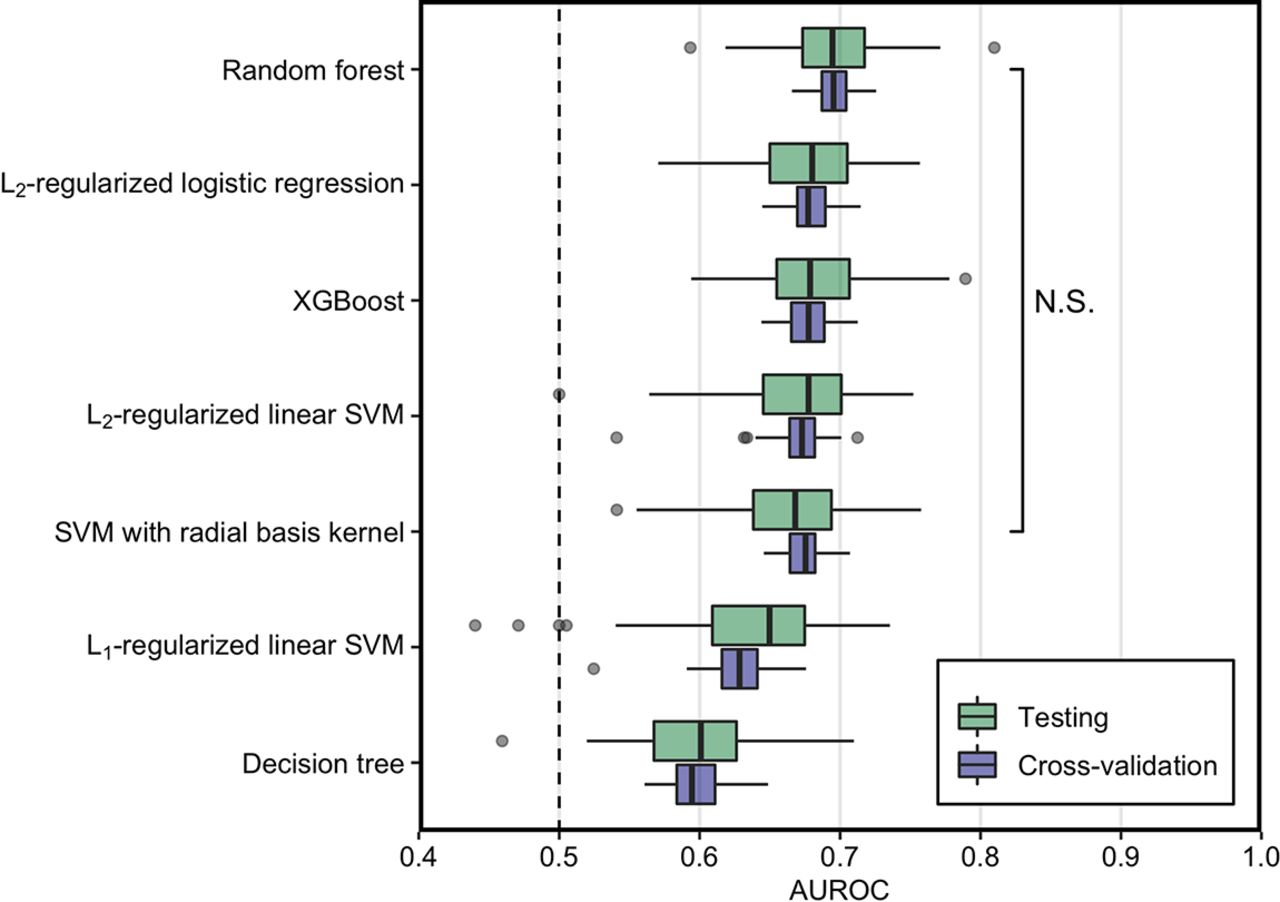
\includegraphics[width=0.5\textwidth]{figures/topcuoglu_f2.jpg}
        \caption{Performance of ML models using AUROC values of cross-validation and testing performances for classifying individuals with SRN (adenoma or carcinoma) using OTU abundances. The performance of random forest was higher than other models, but not significantly (P > 0.05). The vertical line at $0.5$ depicts an AUROC which performs no better than random. \cite{topcuoglu_framework_2020}}
        \label{fig:rf}
    }
    \vspace{-8pt}
\end{wrapfigure}
Binary random forest models will be built to classify samples as CRC or non-cancerous using OTU abundances, metabolic pathway abundances, or both as model features.
The random forest method has been found to perform well for microbiome-based classification problems because it can be used for non-linear data and accounts for interactions between features \cite{baxter_microbiota-based_2016}.
A more recent study comparing modeling methods for OTU-based classification of screen relevant neoplasia (SRN; includes adenoma and carcinoma) found that random forest performed better than other methods including logistic regression, but not significantly so (see Fig. \ref{fig:rf}) \cite{topcuoglu_framework_2020}.
Prior to training, features will be filtered to remove any OTUs and pathways with near-zero variance, as these are not likely to be informative and would only increase training time.
The dataset will be randomly split into 80\% training and 20\% testing sets, stratified to maintain the proportion of CRC to non-cancerous samples.
The mtry hyperparameter, which is the number of features used in each tree split, will be tuned to maximize the mean area under the receiver operating characteristic curve (AUROC) with 5-fold cross-validation.
ROC plots the true positive rate over the false positive rate, while AUROC is interpreted as the chance of classification accuracy.
Each model will then be trained with the best mtry value and the test AUROC will be calculated with the held-out test data.
These steps will be repeated for 100 iterations with a different training/testing data split each time, and the test AUROCs will be recorded.
The statistical significance of differences in mean AUROCs between the three types of models will be evaluated with a pairwise Wilcoxon test with Bonferroni-corrected $P$ values for comparisons among the three models \cite{hannigan_diagnostic_2018}.
The Wilcoxon test is appropriate because for each data split, there is a mean AUROC for each model, thus the mean AUROCs are matched by data splits.
Permutation importance will be performed to determine which features (OTUs and pathways) have the greatest influence over model performance, which implies their importance as CRC biomarkers.
These methods have been lauded as best practices for building OTU-based machine learning models \cite{topcuoglu_framework_2020} and are currently being implemented in an R package (https://github.com/SchlossLab/mikRopML).
To reduce the runtime, these tasks will be run in parallel where possible on the Great Lakes HPC cluster.

\subsection*{Aim 2. Integrating active metabolites with functional gene potential}

\paragraph{2A) Annotate known products of bacterial metabolism from untargeted mass spectrometry.}

Untargeted liquid chromatography tandem mass spectrometry (LC-MS/MS) will be performed on stool samples to determine the functions actively performed by the bacterial community.
LC-MS/MS spectra will be processed with the Global Natural Products Social Molecular Networking (GNPS) a popular web-based tool for processing, annotating, and sharing tandem mass spectrometry data \cite{wang_sharing_2016}.
GNPS queries spectra against all reference spectra accumulated in GNPS libraries to find near-exact matches and annotate known compounds at Level 2 or 3 (Level 1 is only possible by confirming with commerical standards) \cite{aron_reproducible_2020}.
As of 2016, GNPS had 18,163 compounds in its database, and trained users can contribute new spectra created from high quality standards \cite{vargas_protocol_2019}.
The spectral search outputs structures of known annotated metabolites represented by spectra, which will be converted to International Chemical Identifiers (InChi) through the GNPS API for compatibility with the MetaCyc database.
It is important to note that stool samples contain metabolites which can be derived from host metabolism, microbial metabolism, both, or neither.
The functional potential from metagenomes provides an avenue to identify which metabolites are likely products of microbial metabolism.

\paragraph{2B) Find overlapping pathways from active metabolites and functional potential profiles.}

\begin{wrapfigure}{R}{0.4\textwidth}
    %\vspace{-11pt}
    \centering{
        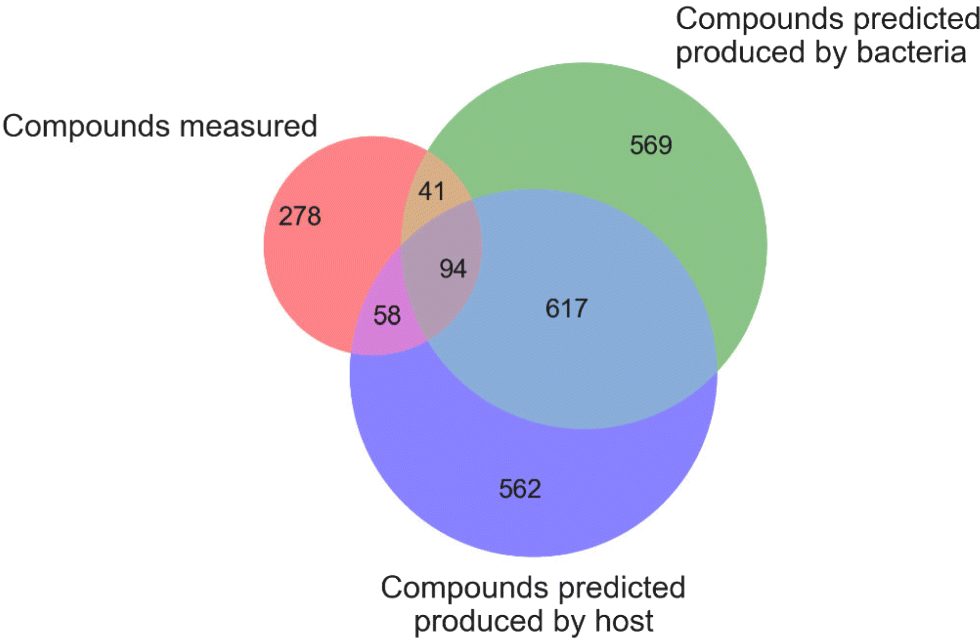
\includegraphics[width=0.4\textwidth]{figures/amon_f2b.png}
        \caption{A case study of applying AMON to identify sources of metabolites in a microbiome sample. The method proposed here will use pathways from MetaCyc identified with HUMAnN2 rather than KEGG, and would result in confirming $41+94=135$ active microbial metabolites if this example dataset were used. \cite{shaffer_amon_2019}}
        \label{fig:amon}
    }
    \vspace{-8pt}
\end{wrapfigure}
The IDs of metabolic products of all pathways encoded in the metagenomes of each microbial community (functional potential profiles) will be queried from the MetaCyc database to create a set of potential metabolites.
The set of potential metabolites will be intersected with the set of metabolites annotated in LC-MS/MS.
The intersection of these sets represents known metabolites which are 1) known to be products of bacterial metabolism in general and 2) capable of being produced by members of these specific microbial communities.
This set intersection would exclude metabolites that are not known to be capable of being produced by microbes, i.e. any metabolites that are only produced by human metabolism or from outside sources such as the host diet (Fig. \ref{fig:amon}).
This method is inspired by AMON, which uses KEGG KOs rather than the MetaCyc database to putatively annotate the origins of metabolites in integrated metagenomic and metabolimic experiments \cite{shaffer_amon_2019}.
MetaCyc will be used here because it is already integrated with the HUMAnN2 tool for profiling functional potential,
it contains more metabolic pathways than the KEGG database,
and the KEGG database can no longer be downloaded in its entirety for free \cite{caspi_metacyc_2020}.

\paragraph{2C) CRC classification models with potential or confirmed active pathways.}

Binary random forest models to classify samples as CRC or non-cancerous will be built in a similar manner as described in Aim 1C, but with model features as potential metabolic pathways identified by HUMAnN2 or using only confirmed active metabolic pathways confirmed with LC-MS/MS.
Features will be coded as binary variables with $1$ for pathway presence and $0$ for pathway absence.
Presence/absence will be used rather than relative abundance because abundaces of potential pathways as determined by HUMAnN2 are based on gene sequence abundances, which is fundamentally different from metabolite quantitation performed in mass spectrometry.
Best practices for model training and evaluation will be performed as described above including splitting training and testing data, tuning the mtry hyperparameter with 5-fold cross validation, calculating AUROCs of each model on the held-out test data, and repeating these steps for 100 iterations.
The statistical significance of differences in mean AUROC between the two types of models will be evaluated with a Wilcoxon test.
Finally, permutation importance will be performed to determine which metabolic pathways were most important for classification model performance.
If the mean AUROC is significantly higher for models using only confirmed active pathways than those using functional pathways,
functional potential on its own is not sufficient to characterize true community function in CRC.
On the other hand, if models using potential pathways perform at least as well as models using only confirmed active pathways,
functional potential may compensate for metabolites missed by mass spectrometry.

\section*{Potential Outcomes and Conclusions}

If the performance of the models using functional potential profiles is significantly better than the model using only taxonomic composition profiles,
that would support the idea that functional redundancy explains the phenomenon of high interpersonal variability in microbiome composition obscuring differences between disease states.
However, if no evidence for functional redundancy is found in Aim 1B, alternative explanations will be required.
Performing feature permutation importance will then be especially necessary in order to identify which functions and/or OTUs are most important in accurate classification and to explain model performance.
If models with functional potential perform no better or worse than taxonomic models,
a possible explanation is that functional potential is not a close enough approximation to true function to discriminate disease states.
In that scenario, validating potential functions with active metabolites will be especially important.

One limitation of this study is that stool samples are only proxies for the actual gut environment.
Not all microbes or metabolites in the gut make it to the stool.
However, stool is preferable because it is far less invasive to provide a stool sample than to undergo colonoscopy.
Also, the data are not time-series.
Each patient only provides one stool sample, and we do not have information on the timing of the bowel movement such as following fasting, eating, sleep, or time of day.
Microbial metabolism is likely to fluctuate depending on some or all of these factors.
Metabolites could be capable of being produced by microbes, but actually weren't being produced in the community at the time of sampling.
Fluctuations in metabolite production would be entirely unknown, and different stool samples could be provided under very different conditions.
This could negatively impact the ability to identify metabolic markers of CRC and reduce model performance.

Another limitation of this study is that there are numerous microbial genes with unknown functions which would be missed by this study.
Similarly to unknown genes, the vast majority of spectra from untargeted mass spectrometry have unknown identity.
As few as ~2\% of spectra can be annotated in untargeted mass spectrometry experiments \cite{da_silva_illuminating_2015}.
This is a major unsolved problem in untargeted metabolomics because confirming spectra with known commercial standards is time-consuming.
Additionally, LC-MS/MS with data-dependent acquisition (the only type supported by GNPS) captures only the most abundant metabolites that cross a specified threshold \cite{xiao_metabolite_2012}.
This study would miss all metabolites that cannot be annotated via spectral search with the GNPS database, that are not abundant enough to be captured by LC-MS/MS, or that participate in pathways that are encoded by unknown genes.
The pathways that these unknown genes and metabolites participate in could be important in CRC etiology and/or classification,
and excluding them could negatively impact model performance as well as obscure our understanding of the underlying biology.
If models using only active pathways do not perform better than those using all potential pathways in Aim 1C,
the importance of unknown metabolites in CRC is a possible explanation.
Directly using all metabolites instead of collapsing into known pathways could circumvent this problem,
but that would greatly increase the number of ML features and would also necessarily include metabolites of non-microbial origin.

Finally, cost is a plausible explanation for the lack of large datasets containing both metagenomics and metabolomics data.
Depending on the rates charged by metagenomics sequencing and metabolomics core services,
this study could cost anywhere from $50$ thousand to $200$ thousand dollars just to generate the omics data for all $434$ stool samples.
That does not even take into account the cost of analyzing the data, training complex machine learning models on a high performance computing cluster, and the salaries of the researchers who will perform the study.
Despite the cost, a large, high-quality dataset of CRC and non-cancerous stool samples with 16S sequence, metagenomics, and untargeted metabolomics would be incredibly valuable for the field.

\pagebreak
\bibliographystyle{submission/nihunsrt} % downloaded from https://www.latextemplates.com/template/nih-grant-proposal
%\section*{\refname}
\footnotesize{
\bibliography{submission/prelim.bib}
\par}
\end{document}
